\documentclass{standalone}
\usepackage{tikz}
\usepackage{ctex,siunitx}
\setCJKmainfont{Noto Serif CJK SC}
\usepackage{tkz-euclide}
\usepackage{amsmath}
\usetikzlibrary{patterns, calc,3d}
\usetikzlibrary {decorations.pathmorphing,decorations.pathreplacing,decorations.shapes}
\tikzset{label style/.append style={font=\small}}
\begin{document}
\small
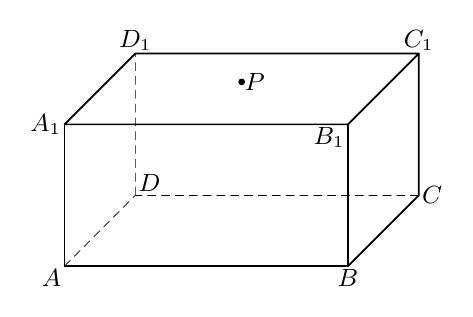
\begin{tikzpicture}[>=latex,scale=0.9,inner sep=1pt]
  \tkzDefPoints{0/0/A,4/0/B,5/1/C,1/1/D,0/2/A',2.5/2.6/P}
  \tkzDefPointsBy[translation=from A to A'](B,C,D){B',C',D'}
  \tkzDrawPoints[fill=black](P)
  \tkzDrawPolygon[semithick](A',B',C',D')
  \tkzDrawSegments[semithick](A,A' B,B' C,C' A,B B,C)
  \tkzDrawSegments[densely dashed](A,D D,D' C,D)
  \tkzLabelPoints[below left](A)
  \tkzLabelPoints[below](B)
  \tkzLabelPoints[above right](D)
  \tkzLabelPoints[right](C,P)
  \tkzLabelPoint[left](A'){$A_1$}
  \tkzLabelPoint[below left](B'){$B_1$}
  \tkzLabelPoint[above](D'){$D_1$}
  \tkzLabelPoint[above](C'){$C_1$}
\end{tikzpicture}
\end{document}